% =========================================================================== %
% Yes. This is a document.

\documentclass[
	ngerman,
	aspectratio=169,
	table
]{beamer}

% =========================================================================== %
% Theme
\usepackage{scrlfile}
	\ReplacePackage{beamerthemeSHUR}{./sty/beamerthemeSHUR}
	\ReplacePackage{beamerinnerthemefancy}{./sty/beamerinnerthemefancy}
	\ReplacePackage{beamerouterthemedecolines}{./sty/beamerouterthemedecolines}
	\ReplacePackage{beamercolorthemechameleon}{./sty/beamercolorthemechameleon}

\usetheme[
	pageofpages=von,
	bullet=circle,
	titleline=true,
	alternativetitlepage=true,
	watermark="",
	watermarkheight=0px,
	watermarkheightmult=0
	]
{SHUR}

% =========================================================================== %
% the usual stuff

\usepackage[utf8]{inputenc}
\usepackage[T1]{fontenc}
\usepackage{babel}
\usepackage{lmodern}
\usepackage{microtype}
\usepackage{csquotes}

\usepackage{tabularx}
\usepackage{booktabs}
\usepackage{multirow}

\usepackage{color, colortbl}
\usepackage{xcolor}
	\definecolor{tabhighlight}{RGB}{230,240,255}

\usepackage{tabto}

\usepackage{minted}
	\usemintedstyle{friendly}

\usepackage{tikz}
	\usetikzlibrary{positioning}
	\usetikzlibrary{matrix}
	\usetikzlibrary{shapes.geometric}
	\usetikzlibrary{backgrounds}
	\usetikzlibrary{calc}
	\usetikzlibrary{decorations.pathreplacing}
	\tikzstyle{every picture}+=[remember picture] 
\usepackage{adjustbox}

\usepackage[most]{tcolorbox}
	\tcbsetforeverylayer
		{colback=cyan!10!white,
		 colframe=cyan!75!black,
		 arc=0pt,
		 outer arc=0pt
		}
	\newtcolorbox{codebox}[1][Code]
		{colback=black!5!white,
		 colframe=blue!40!black,
		 title=#1,
		 leftupper=6mm
		}
	\newtcolorbox{cmdbox}[1][Kommandozeilen-Befehl]
		{colback=black,
		 coltext=white,
		 fontupper=\ttfamily ,
		 colframe=blue!40!black,
		 title=#1,
		 outer arc=0pt
		}
	\newtcolorbox{warnbox}[1][Beachte]
		{colback=black!5!white,
		 colframe=red!40!black,
		 title=#1
		}
	\newtcolorbox{hintbox}[1][Tipp]
		{colback=black!5!white,
		 colframe=green!40!black,
		 title=#1
		}
	\newenvironment{itembox}
		{\begin{tcolorbox}\begin{itemize}}%
		{\end{itemize}\end{tcolorbox}}
	\newtcolorbox{doublebox}[1][.3]
		{righthand width=#1\linewidth,
		 sidebyside,
		 sidebyside gap=6mm,
		 sidebyside align=center,
		 lower separated=false}
	
%==============================================================================%
% GLOBAL MACROS

\newcommand*{\zB}{z.\,B. }
\newcommand*{\ua}{u.\,a. }
\newcommand*{\ie}{d.\,h. }			%% dh is already a defined macro. Couldn't find out what it does.
\newcommand*{\idR}{i.\,d.\,R. }

\newcommand{\Thus}{\ensuremath{\Rightarrow}}
\newcommand{\thus}{\ensuremath{\rightarrow}}

\newcommand*{\tabcrlf}{\\ \midrule}			% actually still allows for optional argument

\newcommand*{\inPy}[1]{\mintinline{python}{#1}}

% =========================================================================== %

\author{Stefan Hartinger}
\title{Programmieren in Python}
\subtitle{Kursteil 5: \texttt{while}-Schleifen und Funktionen}
\institute{Universität Regensburg, Fakultät Physik}
\date{Wintersemester 2020/21}

% =========================================================================== %

\begin{document}
% =========================================================================== %

\begin{frame}[t,plain]
\titlepage
\end{frame}

% =========================================================================== %

\begin{frame}{Recap}
%
\begin{columns}[T]
\column{.5\linewidth}
\begin{itemize}
\item Container
	\begin{itemize}
	\item \inPy{str}ings, \inPy{tuple}s, \inPy{set}s und \inPy{dict}s
	\item (im)mutability, uniqueness, keys
	\item \inPy{range}s -- Zähler
	\end{itemize}
\item \inPy{for}-Schleifen
	\begin{itemize}
	\item \enquote{Für jedes Element aus Container mache...}
	\item Kann verschachtelt werden
	\end{itemize}
\end{itemize}
%
\column{.5\linewidth}
\begin{itemize}
\item List Comprehension
	\begin{itemize}
	\item \inPy{list}s, \inPy{set}s oder \inPy{dict}s schnell aus \inPy{for}-Schleifen erstellen
	\end{itemize}
\item \inPy{enumerate}: Generiere \inPy{tuple}s aus Index und Container-Element
\item \inPy{zip}: Schnüre Datenpakete aus mehreren Containern
\end{itemize}

\end{columns}
%
\begin{center}
	\emph{Noch Fragen?}
\end{center}
%
\end{frame}

% =========================================================================== %

\begin{frame}[fragile]
%
\begin{tcbraster}[raster columns=2,
                  raster equal height,
                  nobeforeafter,
                  raster column skip=0.5cm]
\begin{codebox}[Beispiel: Weihnachtsbaum mit drei Schleifen]
\begin{minted}[fontsize=\scriptsize, linenos]{python}
height = 7

for row in range(height) :
  for column in range(height - row) :
    print(" ", end="")
  for column in range(2 * row + 1)  :
    print("*", end="")
  
  print("")
\end{minted}
\end{codebox}
%
\begin{codebox}[Beispiel: Weihnachtsbaum mit zwei Schleifen]
\begin{minted}[fontsize=\scriptsize, linenos]{python}
height = 7

for   row    in range(    height    ) :
  for column in range(2 * height + 1) :
    f = abs(column - height) < (row + 1)
    
    print("*" if f else " ", end="")
  print("")
\end{minted}
\end{codebox}
\end{tcbraster}
%
\begin{codebox}[Beispiel: Weihnachtsbaum mit einer Schleife]
\begin{minted}[fontsize=\scriptsize, linenos]{python}
height = 7

for row in range(height) :
  print(" " * (height - row - 1), "*" * (2 * row + 1))
\end{minted}
\end{codebox}
%
\end{frame}

% =========================================================================== %

\begin{frame}[fragile]{Gedankliche Schritte -- Analyse und Synthese}
%
\begin{itemize}
\item \emph{Legen Sie eine String-Variable an. Bestimmen Sie, welches Schriftzeichen jeweils wie oft in diesem Text vorkommt.}
\item \emph{jedes Schriftzeichen} \Thus Finde heraus, welche Schriftzeichen vorkommen
	\begin{itemize}
	\item Input: String. Gewünschter Output: Liste von Buchstaben
	\item Betrachte Container-Typen \Thus \inPy{set}: nur einmalige Elemente
	\item Kann aus direkt \inPy{str}ings erstellt werden
	\item[\Thus] Teilaufgabe gelöst
	\end{itemize}
\item \emph{Wie oft diese vorkommen} \Thus Zähle Schriftzeichen
	\begin{itemize}
	\item Wieder: Liste speichern. Zuordnung Schriftzeichen \thus Anzahl \Thus \inPy{dict}
	\item Zählen: Manuell: \inPy{for}-Schleife
	\item Oder Automatisch: Methode \inPy{str.count}
	\end{itemize}
\end{itemize}
%
\end{frame}

% =========================================================================== %

\begin{frame}[fragile]
%
%
\begin{codebox}[Beispiel: Buchstaben Zählen]
\begin{minted}[fontsize=\scriptsize, linenos]{python}
text = "the quick brown fox jumps over the lazy dog"
uniqueChars = set(text)
sortedChars = sorted(uniqueChars)

# manuelle Version
counts = {char : 0 for char in uniqueChars}      # dict mit Startwerten 0 vorbereiten
for char in text :                               # manuell zählen
  counts[char] += 1

# automatische Version
autoCounts = {char : text.count(char) for char in uniqueChars}


print("Analyse von '" + text + "':")
for char in sortedChars :
  print(char, "kommt", counts[char], "mal vor;",
        "automatische Zählung ergibt auch", autoCounts[char])
\end{minted}
\end{codebox}
%
\end{frame}

% =========================================================================== %

\begin{frame}[fragile]{Kapitel 5}
%
\begin{itemize}
\item \inPy{while}-Schleifen
\item Eingriffe in die Schleifen-Struktur
\item \inPy{else} bei \inPy{while} und \inPy{for}
\end{itemize}
%
\end{frame}

% =========================================================================== %

\begin{frame}[fragile]{\inPy{while}-Schleifen}
%
\begin{columns}[T]
\column{.5\linewidth}
\begin{itemize}
\item Grundidee: Wiederhole \emph{[Anweisungen]}, solange Bedingung erfüllt (vgl. menschliche Sprache)
\item Prüfung der Bedingung jeweils \emph{vor} Wiederholung
\item Endlosschleifen möglich
	\begin{itemize}
	\item Kann beabsichtigt sein
	\item Meist aber versehen
	\item Laufenden Code abbrechen:\\
		\texttt{[CTRL] + C} im Konsolen-Fenster
	\end{itemize}
\end{itemize}
%
\column{.5\linewidth}
\begin{codebox}[Syntax: \texttt{while}]
\begin{minted}[fontsize=\scriptsize]{python}
while Bedingung :
    Anweisungen
\end{minted}
\end{codebox}
\end{columns}
%
\end{frame}

% =========================================================================== %

\begin{frame}[fragile]
%
\begin{codebox}[Beispiel: Zinseszins (I)]
\begin{minted}[linenos, fontsize=\scriptsize]{python}
capital  = float(input("Bitte geben Sie Ihr Startkapital ein: "))
interest = float(input("Bitte geben Sie den Zinssatz ein: "    ))
limit    = float(input("Bitte geben Sie Ihr Zielkapital ein :" ))

years    = 0

while capital < limit :
    capital *= 1 + interest
    years   += 1

print("Nach", years, "Jahren ist das Sparziel erreicht.")
\end{minted}
\end{codebox}
%
\end{frame}
% =========================================================================== %

\begin{frame}[fragile]{Eingriff in den Kontrollfluss: \inPy{break}}
%
\begin{itemize}
\item Schleife (\ie \inPy{while} oder \inPy{for}) zu beliebiger Zeit beenden
\item Häufig bei Nebenbedingungen an die Schleife
\item Sinnvollerweise an Bedingung gekoppelt\\
 \Thus \inPy{if}
\item Verschachtelte Schleifen: Verlässt jeweils aktuelle Ebene
	\begin{itemize}
	\item Wenn mehrere Ebenen verlassen werden sollen: Flags benutzen
	\end{itemize}
\end{itemize}
%
\end{frame}

% =========================================================================== %

\begin{frame}[fragile]
\begin{codebox}[Beispiel: \texttt{break} bei einer Ebene]
\begin{minted}[linenos, fontsize=\scriptsize]{python}
count = 0
value = 0

while count < 12 :
    newValue = float(input("Bitte geben Sie einen weiteren Wert ein: "))
    value += newValue
    count += 1
  
    if value > 9000 :
        value = "over nine thousand!!"
        break
  
    print(
        "Bisheriger Gesamtwert nach Eingabe von", count, 
        "Werten:", value
    )

print("Gesamtwert:", value)
\end{minted}
\end{codebox}
\end{frame}

% =========================================================================== %

\begin{frame}[fragile]
\begin{codebox}[Beispiel: \texttt{break} bei mehreren Ebenen]
\begin{minted}[linenos, fontsize=\scriptsize]{python}
import random

total = 0
quitFlag = False

while total < 10 :
    batch = [random.randint(-3, 20) for i in range(5)]
    
    for num in batch :
        print(num, end = ", ")

        if num < 0:
            print("secondary condition: negative number")
            quitFlag = True
            break
        if quitFlag : break
        total += num
    
print("total:", total)
\end{minted}
\end{codebox}
\end{frame}

% =========================================================================== %

\begin{frame}[fragile]{Eingriff in den Kontrollfluss: \inPy{continue}}
%
\begin{itemize}
\item Rest des Schleifenkörpers überspringen
\item Funktioniert auch für \inPy{while} und \inPy{for}
\item Sinnvollerweise an Bedingung gekoppelt \Thus \inPy{if}
\end{itemize}
%
\begin{codebox}[Beispiel: \texttt{continue}]
\begin{minted}[linenos, fontsize=\scriptsize]{python}
container = []
while len(container) < 3 :
    value = int(input("Bitte geben Sie eine gerade Zahl ein: "))
    if value % 2 :
        print(value, "ist ungerade und daher nicht zulässig.")
        continue
    container.append(value)
    print("Bisher eingegeben: ", container)
\end{minted}
\end{codebox}
%
\end{frame}

% =========================================================================== %

\begin{frame}[fragile]{\inPy{else} bei \inPy{while} und \inPy{for}}
%
\begin{columns}
\column{.5\linewidth}
\begin{itemize}
\item Erinnerung: Bei \inPy{while} wird Schleifenkörper nie betreten, wenn Bedingung vor Start nicht erfüllt
\item Optional: \inPy{else} -- Ausführung genau wenn Bedingung vor Start nicht erfüllt
\end{itemize}
%
\column{.5\linewidth}
\begin{itemize}
\item Bei \inPy{for}: Idee \enquote{falls nicht anwendbar}
\item \inPy{else}-Block wird ausgeführt, wenn Schleife \emph{regulär} beendet wird, also nicht durch \inPy{break} abgebrochen wird.
\end{itemize}
\end{columns}
%
\end{frame}

% =========================================================================== %

\begin{frame}[fragile]
%
\begin{codebox}[Beispiel: Zinseszins (II)]
\begin{minted}[linenos, fontsize=\scriptsize]{python}
capital  = float(input("Bitte geben Sie Ihr Startkapital ein: "))
interest = float(input("Bitte geben Sie den Zinssatz ein: "    ))
limit    = float(input("Bitte geben Sie Ihr Zielkapital ein :" ))

years    = 0
while capital < limit :
    capital *= 1 + interest
    years   += 1
else :
    print("Das Startkapital ist bereits groß genug.")
  
print("Nach", years, "Jahren ist das Sparziel erreicht.")
\end{minted}
\end{codebox}
%
\end{frame}

% =========================================================================== %

\begin{frame}[fragile]
%
\begin{codebox}[Beispiel: \texttt{for} mit \texttt{break}{,} \texttt{continue} und \texttt{else}]
\begin{minted}[linenos, fontsize=\scriptsize]{python}
tasks = [("hidden", "watch Fullmetal Alchemist"),
         ("open", "work very hard on Python"),
         ("open", "drink all the coffee")]
         
search = ["watch", "work"]

for keyword in search :
    for ID, (state, task) in enumerate(tasks) :
        if state == "hidden" : continue
        if keyword in task :
            print(keyword, "was found in task ID", ID)
            break
    else :
        print(keyword, "was not found in the tasks.")
\end{minted}
\end{codebox}
%
\begin{cmdbox}[Ausgabe: \texttt{for} mit \texttt{break}{,} \texttt{continue} und \texttt{else}]
\begin{minted}[fontsize=\scriptsize]{text}
watch was not found in the tasks.
work was found in task ID 1
\end{minted}
\end{cmdbox}
%
\end{frame}

% =========================================================================== %

\begin{frame}[fragile]{Kapitel 6}
%
\begin{itemize}
\item Funktionen
\item By-Value- und By-Reference-Parameter
\item Scopes
%\item Optionale Parameter
%\item Variadische Funktionen
%\item Lambdas
%\item Funktionen als Rückgabewert
\end{itemize}
%
\end{frame}

% =========================================================================== %

\begin{frame}[fragile]
%
\begin{columns}[T]
\column{.5\linewidth}
\begin{Large}
{Funktionen}
\vspace{6pt}
\end{Large}
\begin{itemize}
\item Idee: Häufige Arbeitsschritte zu einer Einheit zusammenfassen
\item Können parametrisiert werden (Beispiel: Text in Box ausgeben)
\item Können Ergebnis berechnen (\Thus \emph{Funktion} im mathematischen Sinn)
\item \inPy{return}: Verlasse die Funktion, springe zur aufrufenden Stelle zurück
\inPy{return Ergebnis}: Springe zurück, melde ein Ergebnnis
\item Ohne \inPy{return}: Zurückspringen nach letzter Anweisung
\end{itemize}
%
\column{.5\linewidth}
\begin{codebox}[Syntax: Definition von Funktionen]
\begin{minted}[fontsize=\scriptsize]{python}
def Funktionsname (Parameterliste) :
    Anweisungen
    return Ergebnis
\end{minted}
\end{codebox}
%
\begin{codebox}[Syntax: Funktionsaufruf]
\begin{minted}[fontsize=\scriptsize]{python}
Funktionsname(Parameterliste)
Variable = Funktionsname(Parameterliste)
\end{minted}
\end{codebox}
%
\begin{hintbox}[Reihenfolge]
Funktionen müssen \emph{vor} dem ersten Aufruf definiert sein.
\end{hintbox}
\end{columns}
%
\end{frame}

% =========================================================================== %

\begin{frame}[fragile]{Parameterliste}
%
\begin{itemize}
\item Funktion verwaltet \emph{neue lokale Variable(n)}, die als Startwert die Werte an der aufrufenden Stelle erhalten
\item In Definition: Durch Kommata getrennte Variablennamen
\item In Aufruf: Durch Kommata getrennte Ausdrücke
\item Erste Vorstellung: Arbeitskopie der \emph{ausgewerteten} Ausdrücke wird in lokale Funktions-Variablen gespeichert
\end{itemize}
%
\begin{tcbraster}[raster columns=2,
                  raster equal height,
                  nobeforeafter,
                  raster column skip=0.5cm]
\begin{codebox}[Beispiel: Wertentwicklung]
\begin{minted}[fontsize=\scriptsize, linenos]{python}
def func(x, y) :
   print(x, y)
   x, y = 5, 5
   print(x, y)

x = 3
func(x, x + 5)
print(x)   
\end{minted}
\end{codebox}
%
\begin{tcolorbox}[title=Bild der Speicherstellen]
\scriptsize
\begin{tabular}{l|ccc}
Zeile & $x_{main}$ & $x_{func}$ & $y_{func}$ \tabcrlf
6 & 3 & -- & -- \\
2 & 3 &  3 &  8 \\
3 & 3 &  5 &  5 \\
4 & 3 &  5 &  5 \\
8 & 3 & -- & --
\end{tabular}
\end{tcolorbox}
\end{tcbraster}
%
\end{frame}

% =========================================================================== %

\begin{frame}[fragile]
%
\begin{codebox}[Beispiel: Exponentialfunktion als Funktion]
\begin{minted}[linenos, fontsize=\scriptsize]{python}
def expFunction(x0) :
    x           = 1.0
    denominator = 1.0
    result      = 1.0
    iterations  = 10
    for k in range(1, iterations) :
        x            *= x0
        denominator  *= k
        result += x / denominator
    return result

EulersNumber = expFunction(1.0)             # Aufruf, Speichern in Variable
print(f"Eulers Number is {EulersNumber}")
print(f"e³ = {expFunction(3.0)}")           # Weitergabe an andere Funktion
\end{minted}
\end{codebox}

\begin{cmdbox}[Ausgabe: Exponentialfunktion als Funktion]
\begin{minted}[fontsize=\scriptsize]{text}
Eulers Number is 2.7182815255731922
e³ = 20.063392857142855
\end{minted}
\end{cmdbox}
%
\end{frame}

% =========================================================================== %

\begin{frame}[fragile]
%
\begin{codebox}[Beispiel: Funktion \enquote{ohne} Rückgabewert]
\begin{minted}[linenos, fontsize=\scriptsize]{python}
import math

def printBoxed(text, boxSize) :
    lenText     = len(text)
    countSpaces = boxSize - lenText - 2        # 2 spaces for |borders|
    spacesLeft  = math.floor(countSpaces / 2)  # round down
    spacesRight = math.ceil (countSpaces / 2)  # round up
    print("+" +               (boxSize - 2) * "-"           + "+")
    print("|" + spacesLeft * " " + text + spacesRight * " " + "|")
    print("+" +               (boxSize - 2) * "-"           + "+")
reVal = printBoxed("Don't forget to be awesome!", 60)
print("The function returned:" , reVal)
\end{minted}
\end{codebox}

\begin{cmdbox}[Ausgabe: Funktion \enquote{ohne} Rückgabewert]
\begin{minted}[fontsize=\scriptsize]{text}
+----------------------------------------------------------+
|               Don't forget to be awesome!                |
+----------------------------------------------------------+
The function returned: None
\end{minted}
\end{cmdbox}
%
\end{frame}

% =========================================================================== %

\begin{frame}[fragile]{By-Value und By-Reference-Parameter}
%
\begin{itemize}
\item Funktion \enquote{weiß nicht}, wo original-Information liegt (\emph{kein} pass by reference)
\item Vorstellung: Parameterübergabe als Arbeitskopie (pass by value) -- nur bedingt richtig
\item Tatsächlich: Arbeitskopie von \emph{Adressen}
\end{itemize}
%
\begin{tcbraster}[raster columns=2,
                  raster equal height,
                  nobeforeafter,
                  raster column skip=0.5cm]
\begin{codebox}[Beispiel: Übergabe von Referenz by Value]
\begin{minted}[fontsize=\scriptsize, linenos]{python}
def foobar(data) :
    data.append(1)
    data = data + [2]
    print("in foobar: data =", data)
data = []
foobar(data)
print("on module level: data =", data)
\end{minted}
\end{codebox}
%
\begin{cmdbox}[Ausgabe: Übergabe von Referenz by Value]
\begin{minted}[fontsize=\scriptsize]{text}
in foobar: data = [1, 2]
on module level: data = [1]
\end{minted}
\end{cmdbox}
\end{tcbraster}
%
\end{frame}

% =========================================================================== %

\begin{frame}[fragile]
%
\begin{tcolorbox}[title=Speicherbild]
\begin{center}
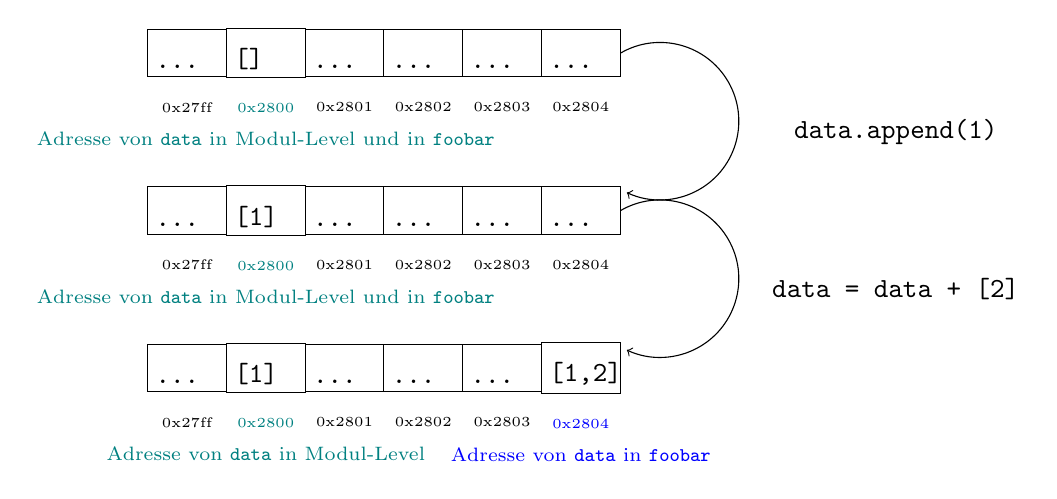
\begin{tikzpicture}
  [ 
    cell/.style={text width=8mm,
      text height=4mm, draw=black, inner sep=1mm},
    ld/.style={draw=blue,shorten >=2pt,->}
  ]
  \node (a1) at (0,4) [cell] {\ttfamily ...};
  \node (a2) at (1,4) [cell] {\ttfamily  []};
  \node (a3) at (2,4) [cell] {\ttfamily ...};
  \node (a4) at (3,4) [cell] {\ttfamily ...};
  \node (a5) at (4,4) [cell] {\ttfamily ...};
  \node (a6) at (5,4) [cell] {\ttfamily ...};

  \node (b1) at (0,2) [cell] {\ttfamily ...};
  \node (b2) at (1,2) [cell] {\ttfamily [1]};
  \node (b3) at (2,2) [cell] {\ttfamily ...};
  \node (b4) at (3,2) [cell] {\ttfamily ...};
  \node (b5) at (4,2) [cell] {\ttfamily ...};
  \node (b6) at (5,2) [cell] {\ttfamily ...};

  \node (c1) at (0,0) [cell] {\ttfamily ...};
  \node (c2) at (1,0) [cell] {\ttfamily [1]};
  \node (c3) at (2,0) [cell] {\ttfamily ...};
  \node (c4) at (3,0) [cell] {\ttfamily ...};
  \node (c5) at (4,0) [cell] {\ttfamily ...};
  \node (c6) at (5,0) [cell] {\ttfamily [1,2]};

%  \node (labelMem) at (8,  1) {Symbole im Code};
%  \node (labelMem) at (8,  0) {Werte im Speicher};
%  \node (labelMem) at (8, -1) {Adressen};
  
  \node (A1) [below=2mm of a1]             {\tiny 0x27ff};
  \node (A2) [below=2mm of a2, color=teal] {\tiny 0x2800};
  \node (A3) [below=2mm of a3]             {\tiny 0x2801};
  \node (A4) [below=2mm of a4]             {\tiny 0x2802};
  \node (A5) [below=2mm of a5]             {\tiny 0x2803};
  \node (A6) [below=2mm of a6]             {\tiny 0x2804};
  
  \node (B1) [below=2mm of b1]             {\tiny 0x27ff};
  \node (B2) [below=2mm of b2, color=teal] {\tiny 0x2800};
  \node (B3) [below=2mm of b3]             {\tiny 0x2801};
  \node (B4) [below=2mm of b4]             {\tiny 0x2802};
  \node (B5) [below=2mm of b5]             {\tiny 0x2803};
  \node (B6) [below=2mm of b6]             {\tiny 0x2804};
  
  \node (C1) [below=2mm of c1]             {\tiny 0x27ff};
  \node (C2) [below=2mm of c2, color=teal] {\tiny 0x2800};
  \node (C3) [below=2mm of c3]             {\tiny 0x2801};
  \node (C4) [below=2mm of c4]             {\tiny 0x2802};
  \node (C5) [below=2mm of c5]             {\tiny 0x2803};
  \node (C6) [below=2mm of c6, color=blue] {\tiny 0x2804};



  \node (main1) [below=0mm of A2, color=teal] {\scriptsize Adresse von \texttt{data} in Modul-Level und in \texttt{foobar}};
  \node (main2) [below=0mm of B2, color=teal] {\scriptsize Adresse von \texttt{data} in Modul-Level und in \texttt{foobar}};
  \node (main3) [below=0mm of C2, color=teal] {\scriptsize Adresse von \texttt{data} in Modul-Level};
  \node (func)  [below=0mm of C6, color=blue] {\scriptsize Adresse von \texttt{data} in \texttt{foobar}};
  
  \draw [->] (a6.east)arc(120:-115:1.0);		%start angle: stop angle : radius  
  \node (step1) at (9,3) {\texttt{data.append(1)}};
  \draw [->] (b6.east)arc(120:-115:1.0);
  \node (step1) at (9,1) {\texttt{data = data + [2]}};
\end{tikzpicture}
\end{center}
\end{tcolorbox}
%
\end{frame}

% =========================================================================== %

\begin{frame}[fragile]
%
\begin{codebox}[Beispiel: Übergabe von Immutables]
\begin{minted}[linenos, fontsize=\scriptsize]{python}
def foobar(data) :
    data = 2
    print("in foobar: data =", data)

data = 1
foobar(data)
print("on module level: data =", data)
\end{minted}
\end{codebox}

\begin{cmdbox}[Ausgabe: Übergabe von Immutables]
\begin{minted}[fontsize=\scriptsize]{text}
in foobar: data = 2
on module level: data = 1
\end{minted}
\end{cmdbox}
%
\end{frame}

% =========================================================================== %

\begin{frame}{Scopes}
%
\begin{itemize}
\item Funktions-Code ist vom übrigen Code \enquote{abgetrennt}
\item Variablen einer Funktion existieren nur lokal
\item Sprechweise: Funktion hat seinen eigenen \emph{Scope}, Variablen gehören zu (leben in) einem Scope.
\item Sehen-Können \enquote{von innen nach außen} aber nicht umgekehrt
\item Parameterliste: Bereits Variablen des Funktions-Scope
\item lokale Neudefinition möglich
\item Aber: Nicht mehr nach dem ersten Lesen
\end{itemize}
%
\end{frame}

% =========================================================================== %

\begin{frame}[fragile]
%
\begin{codebox}[Beispiel: lokale Variablen]
\begin{minted}[linenos, fontsize=\scriptsize]{python}
foo = ["foo"]

def foobar() :
    cat = "confused"      # lokale Variable
    print(foo)            # liest die Variable auf Modulebene
    foo.append("bar")     # schreibender Zugriff, keine Änderung der Adresse
    #foo = foo + ["baz"]  ! Fehler: Neue Adresse

foobar()

print(foo)
# print(cat)            ! Fehler: 'cat' ist Variable von foobar.
\end{minted}
\end{codebox}
\begin{cmdbox}[Ausgabe: lokale Variablen]
\begin{minted}[fontsize=\scriptsize]{text}
['foo']
['foo', 'bar']
\end{minted}
\end{cmdbox}
%
\end{frame}

% =========================================================================== %

\begin{frame}
%
\begin{hintbox}[Abhängigkeiten einfach halten]
Schreibt Funktionen nach den Grundregeln:
\begin{itemize}
\item Einziger \enquote{Daten-Eingang} ist die Parameterliste
\item Einziger \enquote{Daten-Ausgang} ist der Rückgabewert
\item Alle Variablen in Funktionen werden vor dem ersten Lesen mit Startwert definiert (und damit implizit zu lokalen Variablen)
\end{itemize}
Andernfalls werden die Abhängigkeiten sehr konfus, schwer zu warten und anfällig für viele Fehler, da man immer den Zustand des \emph{ganzen Programms} kennen muss.
\end{hintbox}
%
\end{frame}
\end{document}

% MAREI!!
% whom do I give credit? Where?